\documentclass[11pt,a4paper]{article}
\usepackage[T1]{fontenc}\usepackage[utf8]{inputenc}
\usepackage{lmodern,microtype,amsmath,amssymb,amsthm,mathtools}
\usepackage{booktabs,longtable,array,enumitem,xcolor,geometry,fancyhdr,hyperref,graphicx}
\geometry{margin=22mm}
\hypersetup{colorlinks=true,linkcolor=blue!55!black,urlcolor=blue,citecolor=blue!55!black,
 pdftitle={FIN ST1272--ST1361: Frozen OA Dual-Dynamics Discrimination and Composite Robustness},
 pdfauthor={Krzysztof Żuchowski}}
\pagestyle{fancy}\fancyhf{}\fancyhead[L]{FIN ST1272--ST1361}\fancyhead[R]{Release 10.98}\fancyfoot[C]{\thepage}\setlength{\headheight}{14pt}
\newtheorem{theorem}{Theorem}\newtheorem{proposition}[theorem]{Proposition}
\newcommand{\status}[1]{\textsf{[#1]}}

\begin{document}
\begin{titlepage}\centering\vspace*{15mm}
{\Huge\bfseries FIN ST1272--ST1361\par}\vspace{5mm}
{\LARGE Frozen OA Dual-Dynamics Discrimination\par}\vspace{2mm}
{\LARGE and Composite Robustness\par}\vspace{13mm}
{\Large Krzysztof \.Zuchowski\par}
{\normalsize Independent Researcher --- Fractal Information Theory Project\par}
{\normalsize ORCID: 0009-0002-0909-3613\par}\vspace{10mm}
{\large Six research rounds --- 90 programmes\par}
{\large Release 10.98 --- 31 August 2026\par}
\vfill
\begin{minipage}{.87\textwidth}\small
This report freezes one explicitly conditional Operational/State package and
turns the mathematical duality $e^{-tA}$ versus $e^{-itA}$ into an executable
model-discrimination specification.  All finite-count guarantees refer to the
declared ideal hypotheses.  Synthetic fixtures are not experimental evidence.
\end{minipage}\vfill
{\small English mathematical and computational research report.}
\end{titlepage}

\begin{abstract}
Release 10.97 proved that FIN requires an independent operational/state package
$OA$ in addition to conversion and sector packages.  ST1272--ST1361 freeze one
minimal comparison: prepare vertex $0$, evolve with the strict generator $A$,
and measure return to vertex $0$.  The classical hypothesis uses the Markov
semigroup $e^{-tA}$; the quantum hypothesis uses the unitary group $e^{-itA}$.

The return probabilities have exact spectral forms
\[
 C(t)=\frac1{12}\sum_k e^{-\lambda_kt},\qquad
 Q(t)=\left|\frac1{12}\sum_k e^{-i\lambda_kt}\right|^2.
\]
A million-point scan of $0\le t\le10$ together with analytic derivatives finds
the strongest first separation at
$t_*\approx0.59453079$, where
$|Q-C|=0.4112409998$.  This optimization is strong numerical evidence, not an
interval-certified global uniqueness theorem.  The executable protocol freezes
$t=0.6$, losing only approximately $2.3\times10^{-5}$ of the separation.

Under perfect iid preparation and readout, the return event is Bernoulli with
$p_C=0.4123573972$ and $p_Q=0.8235756226$.  An integer likelihood-ratio rule
using 29 clicks and choosing quantum for at least 19 returns gives both errors
below one percent.  Full twelve-vertex readout has Chernoff information
$0.1364798000$, exceeding the binary-return value $0.1002859998$.

The ideal result does not survive arbitrary model broadening.  Energy-basis
dephasing supplies a scalar rate that exactly matches the classical return at
one time; hence a single return probability cannot distinguish classical heat
from the entire open-quantum family.  A frozen four-time design
$(0.3,0.6,1.2,2.0)$ remains separated in a numerical composite fit when the
clock scale is independently constrained to $[0.9,1.1]$.  If the clock scale
is allowed to range over $[0.1,10]$, the open quantum family nearly mimics the
classical curve.  Clock calibration is therefore a necessary input, not an
optional convenience.

The deliverable includes a hashed JSON protocol, a fail-closed validator,
no-click accounting, synthetic positive/negative fixtures and a one-shot
analysis rule.  It does not include apparatus, raw natural events, independent
custody or a laboratory claim.  The result makes dual dynamics falsifiable in
principle under a frozen $OA$ while sharply defining the nuisance-model and
evidence boundaries.
\end{abstract}

\tableofcontents\newpage

\section{Scope and epistemic hierarchy}

This cycle does not attempt to decide the ontology from $A$.  Release 10.96
proved that impossible on the $A$-only datum.  It instead chooses two explicitly
conditional hypotheses inside $OA$ and asks whether their predictions differ.

Four levels are kept separate:
\begin{enumerate}
\item exact finite-model identities;
\item strong numerical optimization or composite fitting;
\item synthetic protocol/validator replay;
\item laboratory evidence, which is absent.
\end{enumerate}

\section{Round I: ST1272--ST1286 --- frozen operational hypotheses}

The common preparation is the selected vertex $0$.  The common coarse
observable asks whether the final vertex equals $0$.

\paragraph{Classical hypothesis $H_C$.}
\[
 p(0)=\delta_0,qquad p(t)=e^{-tA}\delta_0,qquad
 C(t)=(e^{-tA})_{00}.
\]

\paragraph{Quantum hypothesis $H_Q$.}
\[
 \rho(0)=|0\rangle\langle0|,qquad
 U_t=e^{-itA},qquad
 Q(t)=|\langle0|U_t|0\rangle|^2.
\]

Both models use $t=t_{\rm phys}/\tau_*$.  The base hypotheses set dephasing and
loss to zero and fix the clock factor to one.  Those restrictions are part of
the hypothesis, not consequences of $A$.

The full vertex distributions are
\[
 p_x^{C}(t)=(e^{-tA})_{x0},qquad
 p_x^{Q}(t)=|(e^{-itA})_{x0}|^2.
\]
They are normalized and nonnegative.  Circulant symmetry makes all choices of
the source vertex equivalent; this does not produce an absolute origin.

The protocol records a SHA-256 fingerprint of the rounded reconstructed matrix
and freezes the optimization domain $0\le t\le10$ before any future data.

\section{Round II: ST1287--ST1301 --- spectral optimization}

The strict spectrum reduces to seven values with multiplicities
\[
 1,2,2,2,2,2,1.
\]
Consequently,
\[
 C(t)=\frac1{12}\left(1+2\sum_{j=1}^{5}e^{-\lambda_jt}
 +e^{-\lambda_6t}\right)
\]
decreases to $1/12$.  The quantum amplitude is the analogous finite sum of
phases, so $Q(t)$ is almost periodic rather than monotone.

For
\[
 D(t)=|Q(t)-C(t)|,
\]
analytic differentiation gives, with
$a(t)=12^{-1}\sum_ke^{-i\lambda_kt}$,
\[
 Q'(t)=2\operatorname{Re}(\overline a a'),qquad
 Q''(t)=2\bigl(|a'|^2+\operatorname{Re}(\overline a a'')\bigr).
\]
The numerical stationary point is
\[
 t_*\approx0.5945307906,quad
 C(t_*)\approx0.4152434795,quad
 Q(t_*)\approx0.8264844793,
\]
\[
 D(t_*)\approx0.4112409998.
\]
The second derivative of $Q-C$ is negative there.  A grid of $1{,}000{,}001$
points with step $10^{-5}$ finds the same maximum cell.  A global derivative
bound supplies a small cover gap, but floating evaluations are not an outward
interval proof.  The report therefore does not claim an exact unique global
maximizer.

At the practical frozen time $t=0.6$,
\[
 C=0.4123573971501711,qquad
 Q=0.8235756226155311,qquad
 D=0.4112182254653600.
\]
The loss relative to the candidate optimum is about $2.28\times10^{-5}$.

At $t_*$, every nonreturn quantum probability is below its classical
counterpart, so the total-variation distance of the full vertex distributions
equals the return gap numerically.  Later, the sign can reverse because of
unitary recurrence; three positive crossings occur in $(0,10]$ near
$5.6671$, $7.0805$ and $9.7075$.

\begin{figure}[ht]
\centering
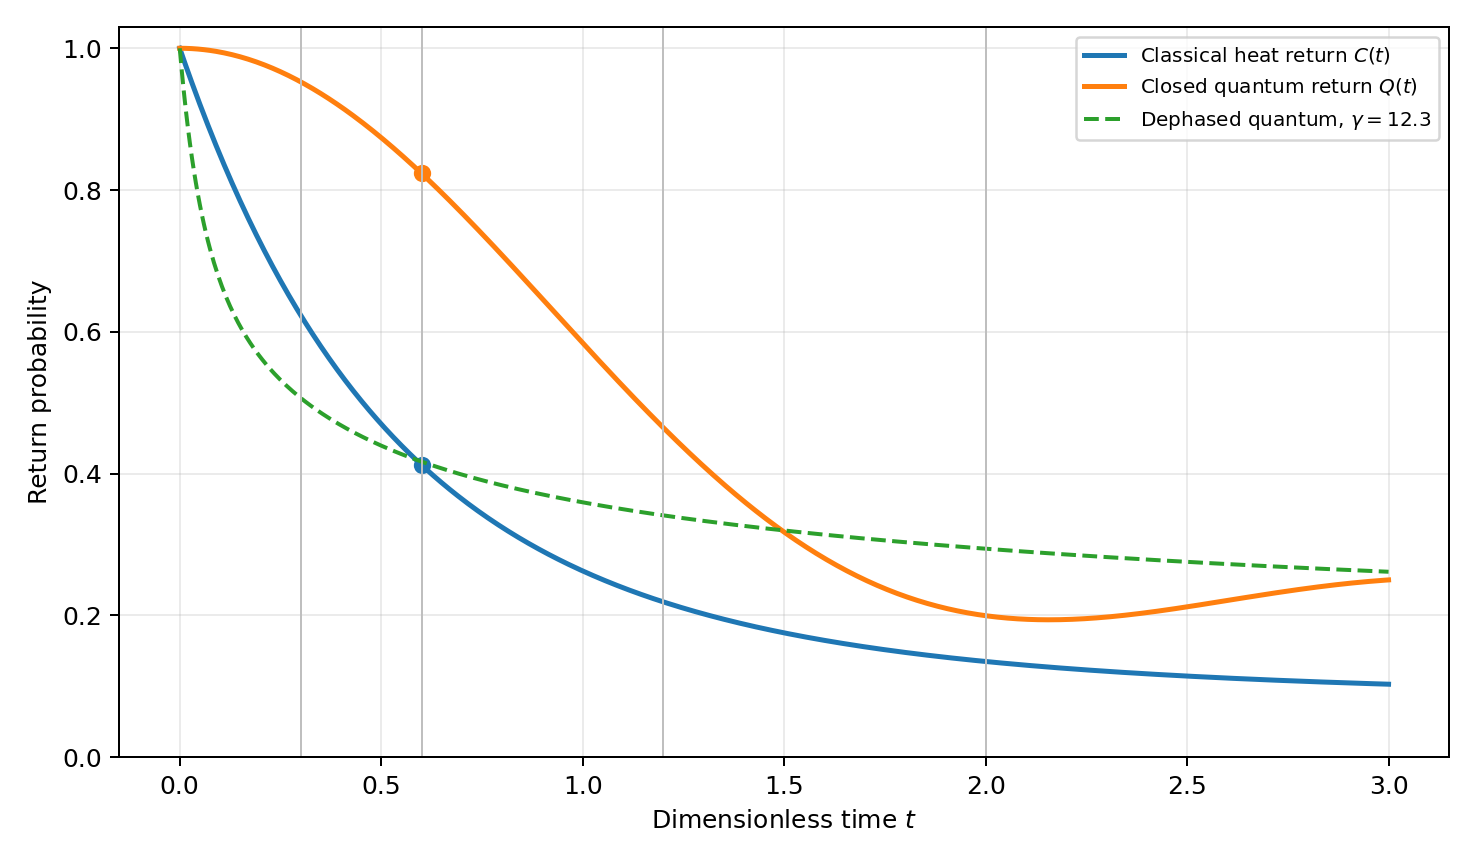
\includegraphics[width=.96\textwidth]{FIN_ST1272_ST1361_Figures/oa_return_discrimination.png}
\caption{Frozen classical and closed-quantum return curves, with one strongly
dephased quantum example.  Vertical lines mark the four-time robust design.}
\end{figure}

\section{Round III: ST1302--ST1316 --- finite counts}

At $t=0.6$, repeated ideal return observations give
\[
 K\sim\operatorname{Binomial}(n,p_C)quad\text{or}\quad
 K\sim\operatorname{Binomial}(n,p_Q).
\]
The directional Kullback--Leibler divergences are
\[
 D(C\|Q)=0.4218128334,qquad D(Q\|C)=0.3574422295,
\]
and the Bernoulli Chernoff information is
$0.1002859998$.  Since $p_Q>p_C$, the likelihood ratio is monotone in the
return count.

\begin{longtable}{@{}p{.18\textwidth}p{.14\textwidth}p{.16\textwidth}p{.20\textwidth}p{.20\textwidth}@{}}
\toprule
Maximum target error & shots $n$ & threshold $k$ & $C\to Q$ error & $Q\to C$ error \\
\midrule\endhead
$5\%$ & 15 & 10 & 0.0420851 & 0.0354013 \\
$1\%$ & 29 & 19 & 0.0071823 & 0.0077975 \\
$0.1\%$ & 48 & 31 & 0.0009280 & 0.0008798 \\
\bottomrule
\end{longtable}

With 100 ideal shots, the best integer threshold gives maximum error below
$4.9\times10^{-6}$.  These are exact binomial-tail calculations in floating
arithmetic, conditional on iid trials, exact preparation, exact time and a
perfect effect.

Retaining the full vertex outcome increases Chernoff information to
$0.1364798000$.  This is expected by data processing: binary return is a
coarse-graining of the multinomial record.

\section{Round IV: ST1317--ST1331 --- nuisance falsification}

\subsection{Clock error}

For the base hypotheses the return gap remains above approximately $0.408$
through a $\pm10\%$ window around $t=0.6$.  Thus moderate timing error alone
does not threaten the ideal separation.

\subsection{Dephasing no-go at one time}

Consider energy-basis dephasing generated by $A$:
\[
 \rho_{jk}(t)=\rho_{jk}(0)
 \exp\left[-i(\lambda_j-\lambda_k)t
 -\frac\gamma2(\lambda_j-\lambda_k)^2t\right].
\]
For a suitable $\gamma\approx12.6$, its return probability at the frozen time
equals the classical return.  Therefore:

\begin{theorem}[single-time composite no-go]
One return probability at one time cannot distinguish strict classical heat
from the family of unitary-plus-free-energy-dephasing quantum models.
\end{theorem}

Strong dephasing does not become classical heat.  Because of spectral
degeneracies its limiting return is
\[
 \frac{1^2+5\cdot2^2+1^2}{12^2}=\frac{22}{144}=0.152777\ldots,
\]
not $1/12$.

\subsection{Four-time composite design}

The robust design freezes
\[
 t\in\{0.3,0.6,1.2,2.0\},qquad100\text{ shots per time}.
\]
Fitting dephasing $0\le\gamma\le100$ and a clock factor
$0.9\le\alpha\le1.1$ gives a best numerical residual sum of squares
$0.0523947$ and maximum point residual $0.1506064$.  This is promising
separation, but differential evolution is not a formal global minimax
certificate.

Allowing $0.1\le\alpha\le10$ reduces the best maximum residual to roughly
$0.0195$.  Thus an independently calibrated clock scale is indispensable.

Uniform detection loss disappears if records are conditioned only on clicks.
The protocol must record attempts and no-clicks.  In a toy uniform vertex-
confusion model, mixing each distribution with the uniform distribution at
rate $\epsilon$ shrinks the gap by $1-\epsilon$.

\section{Round V: ST1332--ST1346 --- executable specification}

The file \path{FIN_ST1332_ST1346_Protocol.json} freezes:
\begin{itemize}
\item the matrix fingerprint and hypotheses;
\item the primary $t=0.6$, $n=29$, $k=19$ rule;
\item the four robust times and 100 shots per time;
\item the clock and dephasing nuisance bounds;
\item raw fields: timestamp, attempt, click/no-click, vertex, configuration and run;
\item invalid-record rules and the one-shot analysis requirement.
\end{itemize}

The dependency-light validator rejects missing fields, inconsistent vector
lengths, noninteger counts, returns exceeding clicks, clicks exceeding attempts,
shot mismatch and missing frozen time.  Invalid data produce \texttt{INVALID},
not a forced classical/quantum verdict.

Seeded synthetic classical and quantum fixtures pass validation and are
classified correctly by the primary rule.  A deliberately invalid fixture
fails closed.  These fixtures test code only; they are not observations.

Provider, registrar and analyst must be distinct; the protocol hash must be
frozen before unblinding.  Local code cannot supply staffed custody roles,
independent holdout or natural events.

\section{Round VI: ST1347--ST1361 --- final verdict}

\begin{longtable}{@{}p{.33\textwidth}p{.22\textwidth}p{.35\textwidth}@{}}
\toprule
Claim & Status & Boundary \\
\midrule\endhead
spectral return formulas & \status{Proven} & finite frozen $A$ \\
large separation near $t=0.595$ & \status{Strong numerical} & no interval global uniqueness \\
29-shot sub-one-percent rule & \status{Proven in ideal model} & iid/perfect OA assumptions \\
full vertex improves Chernoff information & \status{Proven/numerical} & frozen distributions \\
single-time open-quantum identification & \status{Refuted} & free energy dephasing mimics return \\
four-time calibrated composite separation & \status{Strong numerical} & nuisance box, not minimax-certified \\
executable protocol and validator & \status{Constructed/tested} & synthetic fixtures only \\
laboratory discrimination & \status{Absent} & no apparatus/raw events/custody \\
\bottomrule
\end{longtable}

The frozen $OA$ makes FIN's dual dynamics operationally distinguishable in
principle, but only inside a declared model library.  It does not prove that
either channel is nature's dynamics.

The experiment concerns redistribution/mixing versus coherent unitary
evolution inside the proposed total state.  It does not test literal
nonexistence or annihilation of the whole nadsoliton.

\section{Recommended next programmes}

\begin{enumerate}
\item interval-certify the time optimum and stationary-root inventory;
\item solve the exact composite minimax discrimination problem;
\item add state-preparation contamination bounds;
\item add a calibrated detector confusion matrix and drift model;
\item replace the binary statistic by the full multinomial likelihood;
\item derive valid sequential confidence/e-value procedures;
\item certify four-time identifiability over the complete nuisance box;
\item map every $OA$ field to one candidate platform without claiming realization;
\item freeze an independent custody/hash/holdout transfer package;
\item obtain independent laboratory review before collecting data;
\item collect raw event-level records only after protocol freeze;
\item report failure against the predeclared alternative library without model repair.
\end{enumerate}

Stop and return \texttt{INVALID} after a matrix-hash mismatch, clock outside
the calibrated band, unrecorded no-clicks, invalid counts, post-unblinding
model edits or unregistered nuisance mechanisms.

\section{Final conclusion}

\begin{quote}
The dual FIN dynamics is no longer merely a formal analogy after $OA$ is
frozen: it produces sharply different finite probabilities and an executable
test.  The ideal distinction is large.  The scientifically more important
falsification is that one time point cannot identify classical heat against a
reasonable open-quantum family.  Multiple times, calibrated clocks, no-click
records and a frozen nuisance library are necessary.  The resulting protocol
is ready as a mathematical transfer specification, not as experimental
evidence.
\end{quote}

\appendix
\section{Six-round ledger}
\begin{longtable}{@{}p{.18\textwidth}p{.34\textwidth}p{.38\textwidth}@{}}
\toprule
Range & Object & Verdict \\
\midrule\endhead
ST1272--ST1286 & frozen classical/quantum $OA$ & common preparation and return observable \\
ST1287--ST1301 & spectral optimization & near-optimal $t=0.6$, effect $0.4112$ \\
ST1302--ST1316 & finite counts & 29-shot ideal sub-one-percent rule \\
ST1317--ST1331 & nuisance robustness & single-time dephasing no-go; four-time candidate \\
ST1332--ST1346 & executable protocol & hash, validator, no-clicks and fixtures \\
ST1347--ST1361 & synthesis & conditional readiness, no laboratory evidence \\
\bottomrule
\end{longtable}

\section{Reproducibility}
The authoritative result sets run from
\path{FIN_ST1272_ST1286_Results.json} through
\path{FIN_ST1347_ST1361_Results.json}.  Each contains fifteen programmes and
SHA-256 packet references.  The combined test
\path{test_fin_st1272_st1361.py} checks all ninety packets, statistical
thresholds, nuisance status, protocol validation, figure production and
nonpromotion gates.

\section{Nonclaims}
No physical state category, SI clock, apparatus, raw event, independent
custody, laboratory distinction, legacy bridge, selector, Standard Model,
gravity, $L_{\rm total}$ or Theory of Everything is established.  All future
FIN PDFs remain English.

\begin{thebibliography}{9}
\bibitem{cover} T. M. Cover and J. A. Thomas, \emph{Elements of Information Theory}, Wiley.
\bibitem{norris} J. R. Norris, \emph{Markov Chains}, Cambridge University Press.
\bibitem{breuer} H.-P. Breuer and F. Petruccione, \emph{The Theory of Open Quantum Systems}, Oxford University Press.
\end{thebibliography}
\end{document}
